\setcounter{page}{1}
\artigofalse
\chapter{General introduction}
\label{chap:introduction}

\section{Background and motivation}

\subsection{Demand for soil information}

Soil science is experiencing a period of renaissance that started in the last 
decade \cite{HarteminkEtAl2008}. It is a result of a new global demand for soil 
information needed to solve what has been defined as the five major problems of
our time: food security, climate change, environmental degradation, water 
scarcity and threats to the biodiversity \cite{SanchezEtAl2009}. The Food and 
Agriculture Organization (\href{http://www.fao.org/index_en.htm}{FAO}) of the 
United Nations (\href{http://www.un.org/en/}{UN}), through the Global Soil 
Partnership (\href{http://www.fao.org/globalsoilpartnership/en/}{GSP}) project, 
is the main global demander of up-to-date soil information. The objective of 
FAO is to support and ensure the implementation of joint efforts that lead to 
the adoption of sustainable development goals for the soils \cite{FAO2012}. 
Digital soil mapping (DSM), \textit{the} \textit{creation and population of 
spatial soil information systems through the use of field and laboratory 
observational methods, coupled with spatial and non-spatial soil inference 
systems} \cite{LagacherieEtAl2007a}, a branch of pedometrics, a new emerging 
discipline of soil science that corresponds to the \textit{application of 
mathematical and statistical methods for the study of the distribution and 
genesis of soils} \cite{Heuvelink2003}, is the best alternative to meet this 
new demand for soil information. This is because DSM addresses the main 
problems of the classical approach of soil mapping \cite{Kempen2011}. First, 
DSM is data-centered (\textit{environmental-centered}) and gives emphasis on 
producing soil information according to the needs of soil information users 
(\textit{user-driven}). Second, DSM relies on using well documented statistical
models (\textit{reproducible research}) that allow treating the soil as a 
continuum (models of spatial variation). And third, DSM products can be made 
available at a lower cost in soil information systems with quantified 
uncertainty.

Several initiatives have been undertaken around the world in the last years to 
ensure the development and implementation of DSM. The main examples are the 
GlobalSoilMap.net consortium and ISRIC's Global Soil Information Facilities
(\href{http://www.isric.org/projects/global-soil-information-facilities-gsif}{GSIF}).
In Brazil, soil scientists created the Brazilian Network for Research in DSM 
(RedeMDS) with the main objective of generating synergy among Brazilian soil 
scientists to advance the research in DSM in Brazil \cite{RedeMDS2013}. Also, 
the two first job positions for assistant professors in Pedometrics and DSM in 
Brazilian universities were created in 2011 and 2013 \cite{UFRRJ2011,UFSM2012}. 
Unfortunately these local initiatives are not supported by any official 
government demand for up-to-date soil information in Brazil 
\cite{SamuelRosa2012}. Several economic, politic and cultural reasons have been 
pointed out to explain the lack of interest on soil information in Brazil since 
the 1980s \cite{Dalmolin1999, Ker1999, KerEtAl2003, Ramos2003, Espindola2008}, 
but their resolution is out of the scope of this thesis. Alike many other local
initiatives, the present thesis complies with the priorities defined by the 75 
soil scientists from 17 countries that came together in Rio de Janeiro on July 
2006 during the 2nd Global Workshop on Digital Soil Mapping, for whom developing
and implementing DSM depends on training students and experienced soil 
scientists, standardizing methods and measures, and building international 
collaboration \cite{Boettinger2004}.

\subsection{Modern soil mapping} %%%%%%%%%%%%%%%%%%%%%%%%%%%%%%%%%%%%%%%%%%%%%%%%%%%%%%%%%%%%%%%%%%%

Technology plays a determinant role on how we perceive the world around us. When early farmers during the Neolithic Revolution (ca. 10,000 years ago) first observed that soil properties varied in space, they probably saw that such variation was related to other environmental features. This understanding was first formalized using scientific parlance (i.e. mathematization) about 150 years ago \cite{Florinsky2012}, being revisited ca. 75 year ago \cite{Jenny1941}. Today we call this the discrete model of spatial variation, which explains the variation of soil properties in space by creating mutually exclusive units separated by crisp boundaries \cite{Legros2006}. Postwar technological developments in the fields of mathematics, statistics, and informatics, specially in the mining industry, showed that the variation of soil properties could be successfully explained using a continuous model of spatial variation. This model assumes that the spatial variation of soil properties is gradual and depend only on the spatial distances \cite{WebsterEtAl1990}.

In general terms, the DSM framework can be described as a series of seven steps 
as follows:

\begin{description}
  \item [{Step~0}] Identify a reality or problem entity: geographic region where
  pedometric techniques will be used to model the soil property(ies) distribution
  in the geographic and attribute spaces in a given time period;

  \item [{Step~1}] Develop a conceptual model of pedogenesis: verbal 
  representation of the reality or problem entity including the explicit 
  description of soil forming factors and processes that drive soil 
  characteristics and its spatial distribution pattern. This step relies on 
  gathering all environmental information available and applying concepts 
  (expert knowledge) of soil-landscape system, catenary soil development or 
  other theoretical model of explanation of soil spatial variation;

  \item [{Step~2}] Develop a mathematical representation: translate the verbal 
  representation of the reality or problem entity into a set of possible 
  mathematical representations. In this step we use the conceptual model of 
  pedogenesis to define the sample design and the number of soil observations 
  needed to calibrate the DSM model, collect predictor variables from available 
  environmental ancillary data (environmental covariates), specify model 
  structure (linear or non-linear) and define the techniques to be used in the 
  remainder of the DSM modelling activity (tests of independence, normality and 
  homoscedasticity, multicollinearity assessment, variable selection method, 
  goodness-of-fit measures, etc). Several of this tasks can be (and usually are)
  carried out with the aid of a data processing environment such as a computer;

  \item [{Step~3}] Develop a computer representation: translate the set of 
  mathematical representations of the reality or problem entity into a computer 
  representation, that is, a computer code or computer script. The computer 
  code is used to establish the communication between the DSM modeller (a human 
  being) and the data processing environment (a computer) where mathematical 
  representations and DSM model assessment tools are implemented. Developing a 
  computer code that describes all processing steps is at the core of the 
  concept of \textit{reproducible research} in DSM;

  \item [{Step~4}] Data analysis: run the computer code and evaluate the 
  outcomes. This includes the univariate analysis and selection of candidate 
  predictor variables, followed by its multivariate analysis, and evaluation of
  the adequacy of multivariate model(s), namely check model assumptions, look 
  for interactions between predictor variables, evaluate goodness-of-fit 
  measures and visually assess preliminary soil maps. Best performing DSM 
  model(s) are evaluated regarding their tenability (pedological evaluation) 
  and how well they represent the range of possible mathematical models. 
  Failure in this last assessment means that DSM model(s) have to be adjusted 
  and data analysis rerun, or can simply be discarded;

  \item [{Step~5}] Make predictions: application of best performing DSM model(s)
  to predict soil property values and confidence interval at unvisited locations;

  \item [{Step~6}] Statistical validation: validate the set of DSM models using
  existing independent field data and select the best performing model using a 
  statistical criterion. Best performing DSM model is assumed to be the best 
  mathematical representation of the reality or problem entity under 
  consideration. If previous steps have already allowed selecting a single best 
  performing DSM model, statistical validation is used only to assess model 
  accuracy;
  
  \item [{Step~7}] Reformulate the conceptual model of pedogenesis: selected 
  DSM model and prediction and uncertainty maps can provide new insights about 
  the reality or problem entity, and thus allow reformulating or improving the 
  verbal representation of the conceptual model of pedogenesis;
  
  \item [{Step~8}] Populate spatial soil information systems: point soil 
  observations, prediction and uncertainty maps, and metadata are used to 
  populate a spatial soil information system and made available for inspection 
  through different visualization techniques.
\end{description}

\subsection{Sources of uncertainty} %%%%%%%%%%%%%%%%%%%%%%%%%%%%%%%%%%%%%%%%%%%%%%%%%%%%%%%%%%%%%%%%

Soil-mapping models, like any other model, are nothing more than a gross simplification of reality.
This means that soil-mapping models are unable to explain the spatio-temporal soil variation in 
its entirety, but only a small part of it \citep{Heuvelink1998a}. When we use a soil-mapping model
to produce continuous representations of soil properties across space and/or time, i.e. soil
maps, these continuous representations will inexorably deviate from the ``truth''. What the soil map
presents is our most likely expectation about the soil properties -- not our \textit{certainty}
about them. The deviation from the ``truth'' is what we call \textit{error}. Many examples from the 
soil-mapping literature show that, irrespective of the soil property, soil-mapping models have a 
quite variable predictive performance, usually explaining between 15\% (or less) and (rarely more 
than) 75\% of the spatio-temporal soil variation \citep{MooreEtAl1993, OdehEtAl1994, GesslerEtAl1995, 
McKenzieEtAl1999, GobinEtAl2001, SumflethEtAl2008, SunEtAl2012, ViscarraRosselEtAl2013, 
NussbaumEtAl2014, HenglEtAl2015, GaschEtAl2015, HeungEtAl2016}.

The main reason for a soil map to be in error is that the background knowledge and data used to 
construct the soil-mapping model is very limited -- we have to try our best with the available 
resources. Unless we observe the soil everywhere, which would destroy the soil and render the 
observations useless, no matter how large the volume of data is, or how comprehensive our background
knowledge is, it will never be possible to construct a model that explains the entire complexity of 
the soil \citep{Tukey1997}. This means that our knowledge about the soil, and the world as a whole, 
will always be only partial \citep{Box1993}. Because we cannot eliminate the uncertainty of a soil 
map, they can always be considered as wrong, the difference being that some might be useful 
\citep{Box1976}.

Soil modellers/mappers aim at producing the most accurate representations of the soil given the 
available resources. Thus, a reasonable research program is the identification of the causes for 
soil maps being more or less uncertain. For instance, the error that results from making 
extrapolations and interpolations to predict the soil properties at unvisited locations is an 
important source of uncertainty \citep{HeuvelinkEtAl1999, RefsgaardEtAl2006}. Because modern soil 
mapping is data-centred, these errors are larger the farther we are from the existing 
observations. Thus, the most efficient way of reducing these errors is to increase the number of 
observations and improve the spatial coverage of the mapping region \citep{BrusEtAl2007a}. However, most 
soil-mapping projects must rely on using only soil data produced many years ago \citep{KempenEtAl2009, 
HenglEtAl2014, PoggioEtAl2014, NussbaumEtAl2014, MulderEtAl2016}, when most sampling locations were 
defined based on the tacit knowledge of soil surveyors -- that usually place more samples in complex 
and less known areas \citep{Rossiter2000} -- or other poorly documented criteria.

On the contrary, if the budget of the soil-mapping project includes (additional) sampling, soil 
modellers/mappers have to decide upon the number and spatial configuration of the sample 
\citep{deGruijterEtAl2006, WebsterEtAl2013}. Unfortunately this is not an easy task, except if the 
goal is on modelling/mapping very few soil properties that can be rapidly measured using field 
sensors, and for which a model of spatial (co)variation can be assumed known \citep{MarchantEtAl2006}.
In most cases, several difficult-to-measure soil properties have to be modelled/mapped, many of 
which have a poorly known structure of spatial (co)variation. The chosen spatial sample configuration
has to be appropriate for estimating the spatial trend \citep{HenglEtAl2003a, MinasnyEtAl2006b} and 
the variogram model \citep{WarrickEtAl1987, WebsterEtAl1992, Lark2002}, making spatial predictions 
\citep{YfantisEtAl1987, WalvoortEtAl2010} and, (cross)validating the model/map \citep{BrusEtAl2011}, 
four often conflicting objectives. Besides, one must be careful not to decide upon collecting an 
insufficient or an exaggerated number of samples. Sub-sampling can result in soil-mapping models 
with little utility, while over-sampling can produce modelling benefits that do not outweigh the
sampling costs \citep{vanGroenigenEtAl1999}.

Soil data may not only poorly cover the geographic and/or feature spaces \citep{HenglEtAl2003a}, but
also have significant laboratory and positional errors \citep{NelsonEtAl2011}. Besides, some soil 
properties may naturally contain more errors due to their conceptual definition and analytical 
procedures employed. Take particle-size distribution as an example. First, the errors are propagated
to the fraction obtained by difference (silt). Second, pre-treatments, such as organic matter 
oxidation, can change mineral structure \citep{MikuttaEtAl2005a}. And third, ignoring that the 
particle-size distribution is a compositional datum can introduce bias in the predictions 
\citep{LarkEtAl2007}.

Another important source of uncertainty is the covariates used to calibrate the soil-mapping models.
First, because they contain varying levels of error \citep{HeuvelinkEtAl1989}. These errors derive 
from the various methods of data generation, analytical procedures and, inherent characteristics of 
each site. For example, digital elevation models usually present larger errors in areas with steep 
slopes, rough terrains, and great elevations, and with dense forest cover or urbanized 
\citep{Florinsky1998, Toutin2000, FisherEtAl2006}. Interpolation of elevation data using kriging 
can produce spurious artefacts \citep{HenglEtAl2009} compared to hydrologically consistent 
algorithms \citep{Hutchinson1989}. And stereoscopic correlation techniques produce digital elevation
models with poorer quality than interferometric synthetic aperture radar \citep{HirtEtAl2010}.

Deciding upon which covariates to include in the soil-mapping model is another important source of 
uncertainty. This is specially important now days, when the number of available (uncertain) 
covariates increases every week, many of which possibly being statistically redundant. A 
pedologically sound approach for selecting the covariates consists in eliciting the knowledge of a 
few experts \citep{LarkEtAl2007a}, optimally more than five \citep{MeyerEtAl2001}. An expert is 
every soil modeller/mapper with long practical experience and large pedological, mathematical, and 
statistical knowledge \citep{MeyerEtAl2001}. If the mapping region is unknown to the experts, then
a sound \textit{conceptual model of pedogenesis} must be provided. However, the understanding
about the mapping region may be limited to a point that enables building only a very uncertain 
conceptual model of pedogenesis. For example, a unstable landscape that consistently suffers natural
and/or anthropogenic alterations is geomorphologically more complex than a stable one 
\citep{Schumm1979}. As the landscape is rejuvenated, thus increasing complexity, establishing 
soil-landscape relationships becomes very difficult \citep{StreckEtAl2008}. Similar uncertainty 
in the conceptual model of pedogenesis can arise in very old, stable surfaces that have gone 
through many environmental modifications, but were not affected by Pleistocene glaciations 
\citep{MckenzieEtAl2006}. These landscapes commonly have polygenetic soils that present properties
reflecting today but ancient vegetation and climate \citep{PainEtAl1995, Ker1998}.

A most used approach to select the covariates to enter a soil-mapping model is automated selection.
Because automated selection algorithms are available in most software packages \citep{Harrell2001a}, 
are relatively easy to use \citep{DraperEtAl1971}, deliver satisfactory results, 
\citep{HenglEtAl2004}, and are needed to automate soil-mapping routines \citep{HenglEtAl2014}. The 
main uncertainty here is on which method to use. Some methods analyse all possible combinations of 
covariates. Others simulate the process of natural selection \citep{AndersenEtAl2010}. 
Cross-validation selects covariates that produce the best predictions on test sets 
\citep{GuyonEtAl2003}. Other methods take into account the order in which the covariates are added 
to (forward selection) or removed from (backward elimination) the model \citep{LarkEtAl2007a}. And 
the stepwise method adds and removes covariates until no further addition or removal results in 
significant changes in the model \citep{DraperEtAl1998}. Many other methods exist and have been 
already used in soil-mapping projects \citep{PoggioEtAl2013, NussbaumEtAl2014}. Some prefer to use 
dimensionality reduction techniques to reduce the number of covariates \citep{Massy1965} before 
running the covariate selection algorithm \citep{tenCatenEtAl2011a, HenglEtAl2014}. However, there 
are evidences that the number of problems associated with using automated covariate selection 
methods, and dimensionality reduction techniques, can be greater than the number of advantages 
\citep{FarrarEtAl1967, Jackson1993, Chatfield1995, Edirisooriya1995, Harrell2001a, Jolliffe2002, 
Peres-NetoEtAl2005, LarkEtAl2007a}. The most evident being the fact that each method produces a 
different set of covariates which unnecessarily have any physical or biological relation with the 
soil property being modelled/mapped.
 
Soil modellers/mappers also have to chose the form of model that will be used to model the 
empirical relation between covariates and soil properties. Early soil-mapping projects used 
statistical models that assume a linear relation \citep{MooreEtAl1993, OdehEtAl1994}.
Developments in informatics introduced new forms of modelling this relation. Now days most 
soil-mapping projects employ machine-learning methods such as regression trees, artificial neural 
networks, random forests, support vector machines, among many others \citep{HeungEtAl2016}. The 
main reason being that these non-linear models have a greater ability to capture more complex 
site-specific soil-landscape relations \citep{Grunwald2009}. In fact, the relation between soil 
properties and covariates seldom is completely linear \citep{McKenzieEtAl1999}. Once again, the 
problem is that each model produces a different soil map, although the validation statistics may 
suggest that the differences in their performance are insignificant \citep{HeungEtAl2016}. A solution
is to aggregate the predictions of the many models, but this will not necessarily reduce our 
uncertainty. Besides, machine-learning methods are more difficult to implement and interpret, 
possibly being more prone to error, and can be devoid of any pedological information 
\citep{Grunwald2009}.

As we have seen, the sources of uncertainty in soil-mapping projects are multiple and the list 
presented here is far from being comprehensive -- others will do a better job. The main message
is that we cannot eliminate the uncertainty of a soil map and, as such, our knowledge about the 
soil will always be limited. Despite of this, soil models/maps -- and the entire body of human 
knowledge -- are still needed to guide our every-day actions. So, instead of eliminating uncertainty, 
the real quest is for understanding it and its sources. Because while studying the multiple sources 
of uncertainty -- the \textit{known unknowns} --, instead of bringing them all into light, turning 
them into sources of error which we have a good understanding of -- the \textit{known knowns} --, 
we end up uncovering other sources of error that we were not aware of -- the \textit{unknown 
unknowns} \citep{Wikipedia2015}. If a known (or unknown) unknown happens to become a known known, 
then action can be taken to reduce our uncertainty. For example, if we gain knowledge that a source 
of error has a systematic nature, then a corrective measure can be taken right away.

A most comprehensive way of dealing with the known unknowns is \textit{error propagation analysis}, 
also called \textit{uncertainty analysis} \citep{HeuvelinkEtAl1989, Taylor1997}. This is done taking
our uncertainty into account through the soil-modelling steps, seeing how it propagates, and 
evaluating its impact on the uncertainty of the output soil map. This would allow us identifying the
main source of uncertainty, so that we could try to take corrective measures to improve its quality.
But such an exercise is cumbersome \citep{NelsonEtAl2011}, and the efforts required may not
outweigh the benefits, this being one of the reasons why it is rarely carried out. Another important 
reason for error propagation analysis being unpopular is the common ignorance and lack of 
understanding -- perhaps prejudice -- about error and uncertainty \citep{Wechsler2003, Heuvelink2005}.
But the most important reason might be that statistical packages and data analysis environments do 
not include -- if they ever will or should include -- a simple routine, a button, to run a complete 
uncertainty analysis \citep{HeuvelinkEtAl2006b}.

Since soil maps still are useful, despite being in error, most soil-mapping projects adopt a very
pragmatic approach, and the uncertainty is almost completely ignored \citep{McBratneyEtAl2003, 
ScullEtAl2003}. In other words, we assume that all sources of uncertainty are insignificant. 
Positional and analytical errors are disregarded, covariates are taken as certain, and so on. These 
data are used to calibrate a few models, whose parameters are assumed to be estimated without error 
\citep{DiggleEtAl1998}. The soil-mapping model with the best validation statistics, generally 
chosen using (the optimistic) cross-validation, is selected to make spatial predictions at unvisited
locations \citep{BrusEtAl2011}. Errors in the resulting map are regarded as being due to interpolation
error. Most soil-mapping models will output an estimate of this uncertainty, i.e. a measure of what 
we do not know about the modelled/mapped soil property such as the kriging prediction error variance
\citep{HeuvelinkEtAl1989}. But even such a measure is nothing more than a model of our uncertainty 
whose quality needs proper assessment \citep{Goovaerts2001}. Because soil-mapping models that ignore
the spatial autocorrelation of the prediction errors generally are optimistic about our uncertainty,
i.e. they estimate that we known more than we actually do. And geostatistical models can either 
under- or overestimate the uncertainty depending on the available data and modelling decisions 
\citep{Lark2000a}.

Continually ignoring the uncertainty in soil-mapping projects is quite a dangerous choice 
\citep{HeuvelinkEtAl1999}. It can induce the layman -- and even other scientists -- to think that 
soil modellers/mappers produce perfect, complete answers to soil-related issues. The most likely
consequence is what already happened in the end of the 1980's in most countries when funds for
soil-modelling/mapping research were almost completely extinguished \citep{Basher1997, Dalmolin1999,
Ker1999, Ramos2003, HarteminkEtAl2008, Finke2012}: if the soil map is a perfect representation of 
reality, then once it is done, soil modellers/mappers become useless. Nowadays, many 
software packages and data analysis environments include a basic routine to take into account, at 
least, one source of uncertainty \citep{ChristensenEtAl2002, Papritz2015, RibeiroJrEtAl2015}. If a 
more elaborated, problem-specific software is required, then there is the free and open source 
software community. Free access to the scientific literature is guaranteed by many governments, 
universities, and libraries that spend a significant amount of resources every year on subscriptions
and maintenance of digital repositories. Anyone with a true interest in contributing to the body of 
human knowledge must recognize the urgent need to stop neglecting, perhaps consciously denying, what
we already known -- the \textit{unknown knowns} \citep{Zizek2006}.

\section{Content of the thesis}

\subsection{Objectives and research questions}
\label{sec:objectives}

There are several sources of uncertainty that affect the development of soil-mapping models. Many 
of this sources are known, others are still unknown, and some are disregarded due to our ignorance
(or by convenience). The list given in the previous section is far from comprehensive, but it suggests 
that we face a complex scenario. Accordingly, at the time of writing the research project that
guided the development of the present PhD thesis (2012-2013), it seemed appropriate to aim at evaluating 
the main sources of uncertainty in soil-mapping projects. This required an operational definition, 
which was given based on the observation that, in general, the main decisions made by soil 
modellers/mappers are with regard to the

\begin{enumerate}[label=(\alph*)]
\item calibration observations,
\item covariates, and
\item model structure.
\end{enumerate}

The general objective of evaluating these three mains sources of uncertainty was divided into five 
specific objectives with their respective research questions:

\begin{enumerate}
\item Identify appropriate calibration sample sizes and designs for soil-mapping projects.\newline
Research question: How calibration sample size and design affect which covariates enter the 
soil-mapping model, its prediction accuracy, and the monetary cost of the soil-mapping project?

\item Determine the accuracy of freely available covariates and their suitability to calibrate 
soil-mapping models.\newline
Research question: How accurate are the freely available covariates and how much uncertainty 
reduction in the soil-mapping models is achieved when more detailed covariates are used?

\item Identify appropriate covariate selection methods to build linear soil-mapping models.\newline
Research question: How covariate selection methods affect which covariates enter the soil-mapping 
model and its prediction accuracy?

\item Assess the effect of multicollinearity among covariates on the performance of linear 
soil-mapping models.\newline
Research question: How strongly correlated are the freely available covariates and is prediction 
accuracy improved when they are transformed to their principal components?

\item Identify database scenarios in which non-linear soil-mapping models are more efficient than 
linear soil-mapping models.\newline
Research question: In which database scenarios do non-linear soil-mapping models have better 
performance than linear soil-mapping models?
\end{enumerate}

The main expected result was the definition of a working protocol that would allows the construction
of soil-mapping models while taking into account the main factors that influence their performance. 
The goal was to contribute to national (Brazilian Research Network on Digital Soil Mapping) and 
international (GlobalSoilMap and Global Soil Information Facilities) initiatives, while generating a
significant amount of bibliographic material support the teaching of modern soil-mapping techniques 
in Brazilian universities, which is still incipient these days.

With time it became clear that the five objectives and the expected results were quite ambitious. 
Perhaps, I was overwhelmed by the knowledge of the multiple sources of uncertainty at the same time 
that the demand for soil information was increasing, and felt compelled to develop a very through 
study of the sources of uncertainty. The reason for my mistake is simple: the unknown unknowns and
the unknown knowns. First, a few unknown sources of error were uncovered during the development of 
this study, and I decided to confront them because they were closely linked to the sources that were
originally planned to be studied. There also was my poor of knowledge on some known topics, which 
sometimes took me to the wrong direction, and my blind optimism regarding the available (personal, 
material, financial, and psychological) resources. Finally, I came to learn only late that many 
well known methods of data analysis/processing are not used simply because they are not implemented
in a software package -- programming took a lot of my time. As a consequence of these events, the 
resulting PhD thesis deals only with a modified version of the first and second, and only scratches 
the surface of the third and fifth, above-mentioned specific objectives and their respective 
research questions, i.e.

\begin{enumerate}
\item Determine the suitability of freely available covariates to calibrate soil-mapping models.

	\begin{enumerate}[label=(\alph*)]
	\item Does the use of more detailed covariates result in considerably more accurate soil 
	maps?

	\item How does incorporation of spatial dependence in a soil-mapping model compare to the 
	gain in prediction accuracy obtained with using more detailed covariates?

	\item Are the answers to these research questions consistent across soil properties?
	\end{enumerate}

\item Identify appropriate calibration sample sizes and designs for soil-mapping projects.

	\begin{enumerate}[label=(\alph*)]
	\item Can theoretical and algorithmic improvements on existing spatial sample optimization 
	algorithms improved the performance of soil-mapping models?
	
	\item How suboptimal is it to use a sample configuration that was optimized to a different 
	purpose than that that it is going to be use with?

	\item Is it the predictive performance of a soil-mapping model estimated using a sample 
	configuration optimized using heuristics poorer than that of another soil-mapping model 
	whose parameters were estimated using a sample configuration optimized using an 
	\textit{a priori} knowledge of the model?
	
	\item Is it possible to obtain a sample configuration that is efficient in identifying and
	estimating i) the spatial trend and ii) the variogram model, and iii) making spatial 
	predictions?
	
	\item How does the sample configuration affect the estimated model parameters and thus the
	conclusions that can be drawn under the light of the existing conceptual model of 
	pedogenesis?
	
	\item Are the answers to these research questions consistent across sample sizes and soil 
	properties?
	\end{enumerate}
\end{enumerate}


\subsection{Study area}
\label{sec:intro-study-area}

The study area is located in the southern edge of the plateau of the Paraná Sedimentary Basin, in 
the state of Rio Grande do Sul, Brazil. It consists of a small catchment (about \SI{2000}{\hectare}) 
that represents \SI{60}{\percent} of the entire catchment of one of the water reservoirs of the city
of Santa Maria (\reffig{intro-location}). Climate is subtropical humid without a dry season (Cfa, 
Köppen climate classification), with mean annual temperature of \SI{19.3}{\celsius} -- Summer 
temperatures can reach \SI{>40}{\celsius}, while Winter can have negative temperatures
\citep{HeldweinEtAl2009} --, and mean annual precipitation of \SI{1708}{\milli\metre} well 
distributed throughout the year \citep{Maluf2000}. The rainfall pattern is advanced, which is 
characterized by high intensity at the beginning of the precipitation event \citep{MehlEtAl2001}. 
High intensity rainfalls occur from the end of Spring till the beginning of Autumn 
\citep{MouraBueno2012}. Relief varies between plain (slope between \num{0} and \SI{3}{\percent}) and
mountainous (slope between \num{45} and \SI{100}{\percent}), with enclosed valleys (elevation 
ranging between \num{139} and \SI{475}{\metre} above sea level) that determine rainfall volume and 
radiative flux on different surfaces.

\begin{figure}[!ht]
    \centering
    \begin{minipage}[b]{95mm}
      \subcaption{}
      \label{fig:brazil}
      \centering
      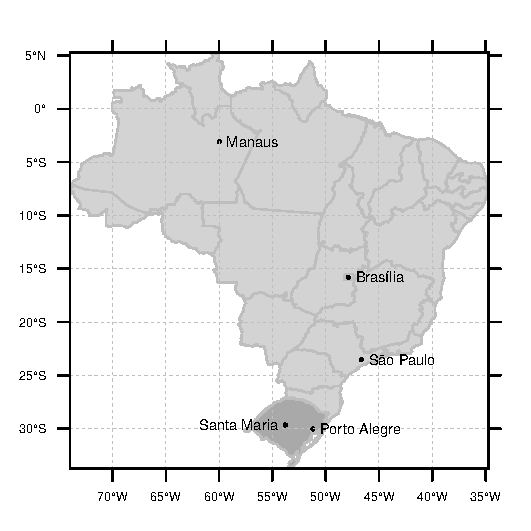
\includegraphics[width=90mm]{chap01FIG1a}
    \end{minipage}
    \begin{minipage}[b]{95mm}
      \subcaption{}
      \label{fig:points}
      \centering
      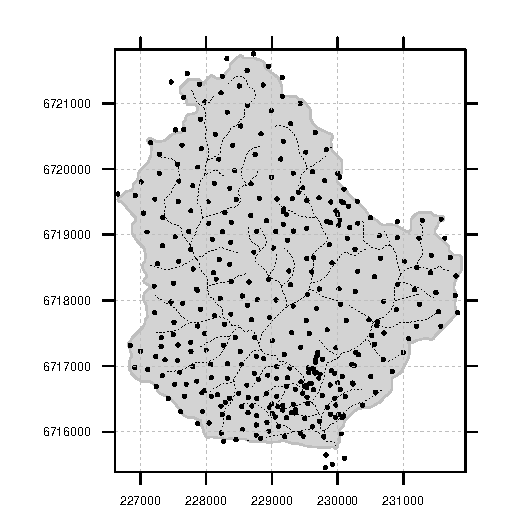
\includegraphics[width=90mm]{chap01FIG1b}
    \end{minipage}
  \caption{The study area. The top panel shows the location of the study area in the central region 
  of the southernmost Brazilian state, Rio Grande do Sul. The bottom panel uses a RapidEye image
  of the year of 2012 in perspective to give an overview of the land use and terrain features.
  A large collection of images of the study area are available at the web-page of the group
  \href{http://www.panoramio.com/group/130903}{Águas do Perau} on Panoramio.}
  \label{fig:intro-location}
\end{figure}

The geology of the study area is composed of three geological formations plus Quaternary deposits
\citep{GasparettoEtAl1988, MacielFilho1990, Sartori2009}.
Consolidated sedimentary rocks (fluvial sandstone -- Caturrita Formation) of the Triassic period 
appear at elevations bellow \SI{\pm200}{\metre}. Basic and acid igneous rocks (andesite-basalt and 
rhyolite-rhyodacite -- Serra Geral Formation) of the Cretaceous period appear at elevations between 
\num{\pm200} and \SI{\pm350}{\metre}, and above \SI{\pm350}{\metre}, respectively. Between these
rocks there are layers of consolidated sedimentary rocks (aeolian sandstone -- Botucatu Formation) 
of the Jurassic period. Unconsolidated colluvial deposits of igneous and sedimentary material eroded
further upslope during the Quaternary period occur at elevations below \SI{\pm300}{\metre}, while 
recent fluvial deposits can be found close to drainages.

Current geomorphology is a result of erosive processes of the Tertiary and Quaternary, wherein the 
landscape sculpting was determined by alternations between humid, semi-arid and arid climates 
\citep{Sartori2009}. Landscape dissection is weak due to the current climate that favours the 
installation and maintenance of an exuberant vegetation \citep{Sartori2009, NascimentoEtAl2010}.
There are three large morphostructural units \citep{GasparettoEtAl1988, NascimentoEtAl2010}:

\begin{enumerate}[label=(\alph*)]
\item the Planalto, with gently-rolling to slopping relief, composed predominately of denudational
 forms with flat surfaces, convex tops, and gently rolling convex slopes, often embedded in faults 
and/or fractures,

\item the Rebordo do Planalto, with wide altimetric variation, steep slopes and abrupt cliffs, composed 
predominately of denudational forms with convex, acute tops, presenting straight slopes with large 
vertical drops often interrupted by terraces, generally embedded in faults and/or fractures, and

\item the Depressão Periférica, composed of aggradational fluvial plains and denudational forms, the
last with convex tops and flat surfaces, presenting concave elongated slopes.
\end{enumerate}

The drainage network has a well defined pattern, generally regular, determined by the faults and/or
fractures \citep{Bortoluzzi1974, GasparettoEtAl1988, NascimentoEtAl2010}. In the lower areas, its
configuration is snake-like due to sediment deposition and fluvial erosion \citep{PaivaEtAl2001, 
SutiliEtAl2009}. Here the plain to gently-sloping, long, concave slopes favour the occurrence of a 
water table close to the surface and the maintenance of perennial water streams. In the upper, 
undulating areas the rectilinear drainage network has little activity in periods of drought. Floods 
are characterized by high flow velocity and volume due to the steep slopes and \SI{\pm120}{\metre} 
vertical drop from the upper to the lower part of the catchment \citep{PaivaEtAl2001, SutiliEtAl2009}.

Land use for agrosylvopastoral production was intense in past times, resulting in severe soil 
degradation. Recent abandonment of many degraded areas allowed the regeneration of natural 
vegetation. The area occupied with forest and secondary vegetation nowadays is \SI{\pm60}{\percent},
specially in difficult to access areas, with steep slopes, shallow and stony soil 
\citep{SamuelRosaEtAl2011a}. Many of these areas are still used for livestock during some periods of
the year, which is negative for natural regeneration \cite{ScheneiderEtAl1978, HackEtAl2005}, and 
are traversed by old and degraded trails that drain rainwater. About \SI{\pm30}{\percent} of the 
area is used for agrosylvopastoral activities year-round, mainly extensive livestock, which relies 
on natural pastures in areas with deeper, less stony soil, and less sloping relief. Only a few 
agrosylvopastoral activities are carried out in areas with steep slops and shallow soil. Urban
settlements occupy only a small portion of the catchment, mainly close to drainages, the largest
settlements being in the southern region.

The soil in the study area started forming during the Triassic and have a strong dependency on the 
parent material \citep{NascimentoEtAl2010}. It is predominantly shallow (\SI{0.5}{\metre}, Neossolo 
and Cambissolo) due to the dominance of steep slopes, which result in soil formation rates being 
close to or lower than soil erosion rates \citep{DalmolinEtAl2006a}. Even in gently-slopping terrain
it is common to find shallow soils as a result of soil degradation \citep{Moser1990, MouraBueno2012}.
Deeper soil (\SI{>1}{\metre}, Argissolo and Planossolo) can be found in the Planalto, in the 
terraces of the Rebordo do Planalto, and in the small hills with gently-rolling slopes and alluvial 
plains of the Depressão Central \citep{Moser1990, MiguelEtAl2012}. Soil texture is finer and more 
homogeneous throughout the soil profile when the soil has developed from igneous rocks, where the 
presence of iron oxides gives a reddish colour to the soil \citep{MiguelEtAl2012}. Soil features in 
the alluvial plains are determined by seasonal or permanent water-logging, sedimentation, or both 
(Planossolo and Neossolo Flúvico). One such feature is the common presence of clay accumulation in
subsurface horizons due to argiluviation, preferential lateral erosion and, possibly, geological
discontinuities \citep{PieriniEtAl2002, MiguelEtAl2012}.

%TODO
\subsection{Database}
\label{sec:intro-database}

The soil database used in this study is part of the 
\hyperref[apen:database]{\textit{Santa Maria dataset}}, a dataset composed of $n = 410$ soil 
observations made between \num{2004} and \num{2013} as part of different research
projects. These projects aimed at producing semi-detailed soil and land use maps (\scale{25000}) 
\citep{Pedron2005, Miguel2010, SamuelRosaEtAl2011a, MiguelEtAl2012, Samuel-RosaEtAl2013}, and 
predicting the vulnerability of the topsoil to erosion \citep{MouraBueno2012, Miguel2013}. 
The Santa Maria dataset, which is freely available at ISRIC World Soil Information Service 
(\href{http://www.isric.org/data/wosis}{WoSIS}) and is fully documented at the end of this thesis
(\autoref{apen:database}), is composed of three subsets, but only two of them are used here 
(\reffig{intro-database}).

\begin{figure}[!ht]
  \centering
  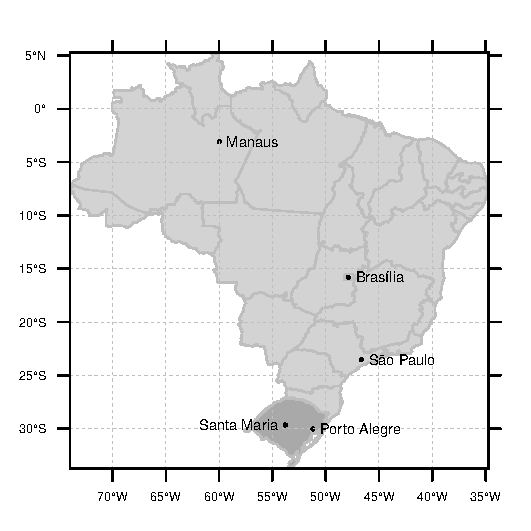
\includegraphics[width=90mm]{chap01FIG1a}
  \caption{Spatial distribution of the $n = 350$ point soil observations used in this thesis.}
  \label{fig:intro-database}
\end{figure}

The first dataset ($n = 340$) was produced using purposively selected observation locations (free 
survey). The main goal of the researchers was to obtain a sample that they understood as being 
representative of the different landforms, land uses, and soil taxa present in the study area. They 
also wanted the sample to cover the entire study area. At the observation locations, they defined 
an area of \SI{\approx100}{\metre\squared} within which they opened three soil pits. Soil samples 
were collected up to a depth of \SI{20}{\centi\metre}. The resulting sampling depth varies from 
\num{2} to \SI{20}{\centi\metre}, with a mean of \SI{17}{\centi\metre}. Soil samples from the three 
pits were used to produce a composite sample which was used for laboratory analysis. Georeferencing 
took place in the field using a GNSS signal receiver with a horizontal precision of more than 
\SI{\pm8}{\metre} positioned approximately at the centre of the sampling area. When the GNSS signal 
was affected by vegetation biomass, terrain features and satellite configuration, resulting in a 
horizontal positional error larger than \SI{\pm8}{\metre}, georeferencing was carried out in the 
office using \SI{1}{\metre} spatial resolution Google Earth satellite images with a positional 
horizontal error of less than \SI{\pm6}{\metre}.

The second dataset ($n = 10$) contains data from the uppermost A horizon of modal soil profiles 
whose location was purposively selected after the observations of the first dataset had been made, 
and a preliminary area-class soil map had been produced. The researchers aimed at locations that 
they understood as being most representative of the soil mapping units depicted in the area-class 
soil map. A single soil sample was taken from the each described soil horizon and used for 
laboratory analysis. The resulting depth of the uppermost A horizons varies from \num{12} to 
\SI{30}{\centi\metre}, with a mean of \SI{22.6}{\centi\metre}. Georeferencing was carried out as 
described above, the difference being that GNSS signal receiver was positioned at the observation 
location.

Four soil properties contained in the Santa Maria dataset are explored in this thesis: clay content
(CLAY, \si{\gram\per\kilo\gram}), organic carbon content (ORCA, \si{\gram\per\kilo\gram}), 
effective cation exchange capacity (ECEC, \si{\milli\mole\per\kilo\gram}), and bulk density 
(BUDE, \si{\mega\gram\per\cubic\metre}). CLAY was 
determined by the pipette method. ORCA was determined using wet digestion. ECEC was calculated as 
the sum of exchangeable bases plus exchangeable acidity. BUDE was determined using the core method. 
The first three of these soil properties were selected because they were expected to present 
different patterns of spatial variation and correlation with the dominant factors of soil formation 
in the study area: organisms (\textit{O}), relief (\textit{R}), and parent material (\textit{P}). 
CLAY was presumed to have a stronger relation with \textit{P}, while ORCA was expected to be more 
correlated with \textit{O}. Because the soils of the study area were strongly eroded due to intense 
agriculture in the 20th century, both CLAY and ORCA were also expected to be closely related with 
\textit{R}. Finally, ECEC was expected to be strongly correlated with \textit{P} and \textit{O}, 
which is supported by its natural relationship with both CLAY and ORCA. BUDE was selected because it
was the only soil property that approximately follows a normal frequency distribution, while the 
other three have a right-tailed frequency distribution (\autoref{intro-soil-properties}). The main 
weakness of the BUDE data is that it is available at only $n = 282$ observations due to soil stoniness.

 \begin{figure}[!ht]
   \centering
    \begin{minipage}[b]{63mm}
      \subcaption{}
      \centering
      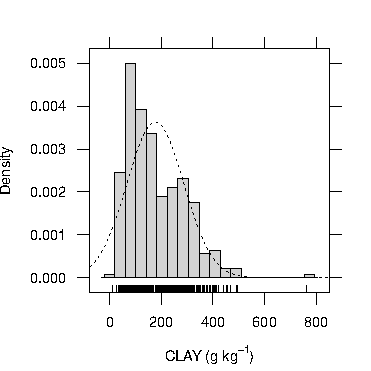
\includegraphics[width=63mm]{chap01FIG2a}
    \end{minipage}
    \begin{minipage}[b]{63mm}
      \subcaption{}
      \centering
      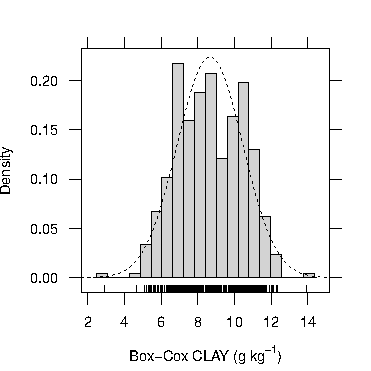
\includegraphics[width=63mm]{chap01FIG2d}
    \end{minipage}
    \begin{minipage}[b]{63mm}
      \subcaption{}
      \centering
      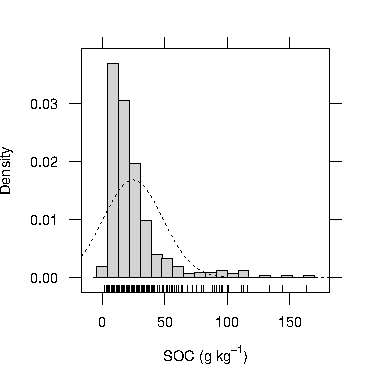
\includegraphics[width=63mm]{chap01FIG2b}
    \end{minipage}
    \begin{minipage}[b]{63mm}
      \subcaption{}
      \centering
      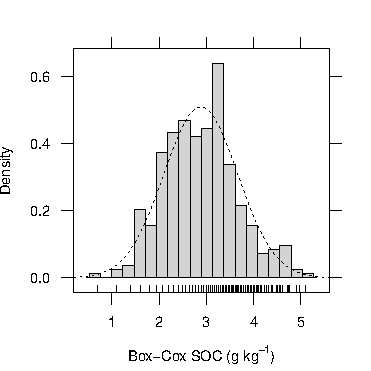
\includegraphics[width=63mm]{chap01FIG2e}
    \end{minipage}
  \caption{The four topsoil properties contained in the Santa Maria dataset explored in this thesis:
  (a) clay content, (b) organic carbon content, (c) effective cation exchange capacity, and (d)
  bulk density. Each panel shows the histogram of frequency, empirical density function, and a few 
  summary statistics.}
  \label{fig:intro-soil-properties}
 \end{figure}

Covariate data include 20 data layers freely available for the study area, 
depicting information on relief, vegetation, land use, geology, soil parent material, soil (taxa) 
and intimately-associated surface conditions.




\subsection{Outline}

This thesis is composed of five chapters: this \textit{General introduction}, where the scope of the
thesis is presented, three core chapters that address the objectives and research questions presented
in \refsec{objectives}, and the last, a \hyperref[chap:conclusion]{\textit{General conclusion}}
of the work that was developed during the last four years. The second chapter (\hyperref[chap:chapter01]{\textit{Chapter
I}}), is based on an article published in the peer reviewed journal 
\href{http://www.journals.elsevier.com/geoderma/}{Geoderma}. The chapter compares linear soil-mapping
 models calibrated using covariates available in two levels of detail, with and without taking the 
spatial dependence of the residuals into account (Questions 1a-c).

The third (\hyperref[chap:chapter02]{\textit{Chapter II}}) and fourth chapters 
(\hyperref[chap:chapter03]{\textit{Chapter III}}) are based on manuscripts submitted to peer 
reviewed journals, both dealing with the second objective of this thesis. The 
former evaluates if improving a popular algorithm used to optimize sample configurations for spatial
trend estimation results in more accurate spatial predictions (Questions 2a and 2f). The last 
compares five methods for designing sample configurations on how they affect estimated model 
parameters and prediction accuracy (Questions 2b and 2e). It also presents an algorithm for 
optimizing sample configurations for identifying and estimating the spatial trend and variogram 
model, and making spatial predictions (Question 2d). Finally, it evaluates the gain in prediction 
accuracy when a sample configuration is optimized assuming the form of the model to be known 
(Question 2c).

This thesis also includes a through description of the soil and covariate databases
(\hyperref[apen:database]{\textit{Appendix A}}), and a verbal representation of the conceptual model
of pedogenesis (\hyperref[apen:pedogenesis]{\textit{Appendix B}}), both summarized above in section
\ref{sec:database}. The third appendix (\hyperref[apen:spsann]{\textit{Appendix C}})  contains a 
description of the \texttt{R}-package \texttt{spsann}, designed for the optimization of sample 
configurations using spatial simulated annealing. Finally, the fourth appendix 
(\hyperref[apen:pedometrics]{\textit{Appendix D}}) presents a description of the \texttt{R}-package
 \texttt{pedometrics}, which includes miscellaneous functions.

All chapters can be read separately, which means that there might be some overlap between chapters, 
i.e. repeated information. However, there are clear links between this introductory chapter 
and the concluding chapter. Chapters II, III, and Appendix C also are closely connected. References 
to specific sections of other chapters are common. All literature references are presented under a
unique \hyperref[chap:references]{\textit{Bibliographic references}} section at the end of this
thesis.
